%\documentclass[12pt]{article}
%\usepackage[margin=1 in, head=0.9 in]{geometry}
%\usepackage{fancyhdr}
%\usepackage{listings}
%\usepackage{caption}
%\usepackage{color}
%\usepackage{xcolor}
%\usepackage{caption, apacite}
%\DeclareCaptionFont{white}{\color{white}}
%\DeclareCaptionFormat{listing}{\colorbox{gray}{\parbox{\textwidth}{#1#2#3}}}
%\captionsetup[lstlisting]{format=listing,labelfont=white,textfont=white}
%\usepackage{graphicx}
%\usepackage{amsmath, amssymb, amsthm}
%\usepackage[all,cmtip]{xy}
%\pagestyle{fancy}
\input{/home/dmitry/Work/Research/thesis/FINALE/settings.tex}

\begin{document}

\title{Gravity wave scattering by large scale sea bottom features}
\maketitle

\section{Abstract}
Oceanic gravity waves fundamentally contribute to redistribution of mechanical energy in the world ocean. Energy transfer from wave generation sites to dissipation regions are controlled by the physics of gravity waves. The energy transfer occurs not only in the lateral direction but also by conversion into vertical movements such as internal waves. For surface and interior fluid motions, interaction with the sea bottom irregularities can alter gravity wave energy pathways. That is energy can be reflected and scattered both in different directions and into propagation modes. My PhD project addresses wave scattering and reflection by sea bottom features in two important cases: a tsunami wave scattered from a prominent sea mount and reflection of a semidiurnal internal tide from a continental slope.\\
Evidently, bottom bathymetry determines local wave behaviour both for barotropic and baroclinic modes. The gravity wave scattering and excitation of subsidiary wave patterns controls energy pathways on the world ocean scales. This thesis intends to investigate physical aspects of wave energy scattering, mode conversion over topographic features and variability in these process.\\
Interactions of tsunami waves with seafloor topography can delay and redirect the energy flux, \textit{creating amplified waves with long periods}. During the March 2011 tsunami event in Japan tide stations in Northern and Central California recorded large waves, while much smaller waves were observed in Washington and in the southern California. This correlated with a ray of high energy originating from the distant scattering from Emperor seamount chain and more specifically from Koko Guyot. This underwater feature focuses energy into tight beams. This investigation shows that guoyt's shape is responsible for the observed signals. The 2011 tsunami event is compared with a case of Kuril tsunami of 2006. The comparative analysis emphasis strong correlation between frequency of incident tsunami wave component, its propagation direction and the observed signal at Northern California.\\
The energy can be distributed not only by surface expression of the sea but also in the ocean's interior. Internal tides originate as surface tide encounters steep topographic feature. At such location the energy would drain into perturbations of isopycnals that further can travel hundreds of  leagues without any significant loss of energy. In the second part of my thesis origination, propagation and dissipation of the internal tidal beam is investigated on the example of Tasman Sea. 
A global internal tide model, satellite altimetry measurements and in situ observations indicate that a ridge south of New Zealand is a site for the generation of the strong tidal beam that is directed towards the Tasman Shelf break. The low mode internal wave beam undergoes scattering from topography, which transfers energy to shorter length scales. Thus, understanding of local energy processes will lead to a more detailed picture of tidal energy dissipation.\\
\textbf{CONCLUSIONS}

\section{Introduction}
Gravity waves are ubiquotous feature of the World Ocean. The fundamental importance of the linear gravity waves is their ability to transfer momentum over large length scales. The energy pathways of propagating gravity waves can be altered in a result of interaction with large scale sea bottom features such as submarine seamountains, trenches and continental shelves. These processes appreciably shape wave propagation, and thus, leading to variation in localized energy budgets. In this work two geophysically important cases are considered. Two examples of energy scattering will be considered in this thesis work.\\
The first deals with tsunami waves (\textbf{HERE IT GOES LONG INTRODUCTION to TSUNAMI WAVE: IMPORTANCE, WHERE IT OCCURS, WHAT IT CAUSES, SECTION?})\\
What is missing? References. More generalization? Decay? Murty, Rabinovich, Kowalik, that Greek lady.
Tsunami waves are transient waves occurring owing to its generation earthquakes along deep ocean trenches (impulsively forced by submarine earthquakes). Rapid uplift of sea bottom creates a hump water that further freely propagates away from the trench in deep ocean. During their transoceanic propagation these waves encounter numerous large scale ocean bottom roughness such as seamount chains and submarine plateaus. All of these obstacles can redirect tsunami propagation because of rapid change in ocean depth. This phenomena is well known as wave refraction in coastal oceanography.\\
For the US it is of most importance understanding how tsunami waves are transformed when their origination lays along Japan-Kuril trench (Figure 1 map. There one of the most disruptive and powerful events in the recorded history occurred. For example, tsunami event happened near Japan on March 12, 2011 created a devasting wave that caused huge along shore run ups in Japan, the wave crossed the Northern Pacific Ocean and caused severe economical losses to the West Coast. In this example it is emphasized that interaction with prolonged chain of seamounts known Emperor Seamount chain has created additional conditions for relatively directive and focused signal on the West Coast.\\
Several previous studies have identified that the primary source of scattering of tsunami waves in Pacific Ocean is Koko Guoyt. Here the secondary waves originate from interaction with steep seamount. Later secondary waves form a distinctive beam which has its final destination towards Mendocino Escarpment where additional focusing occurs bringing amplified waves to Crescent City, CA. In such scenario it is notable that observations suggest arrival of the secondary waves long after the main tsunami wave arrival occurs. Hence, developing understanding of mechanisms behind generation of the scattered tsunami waves have important forecasting consequences. This work is developing a description for such mechanism.\\

\begin{figure}
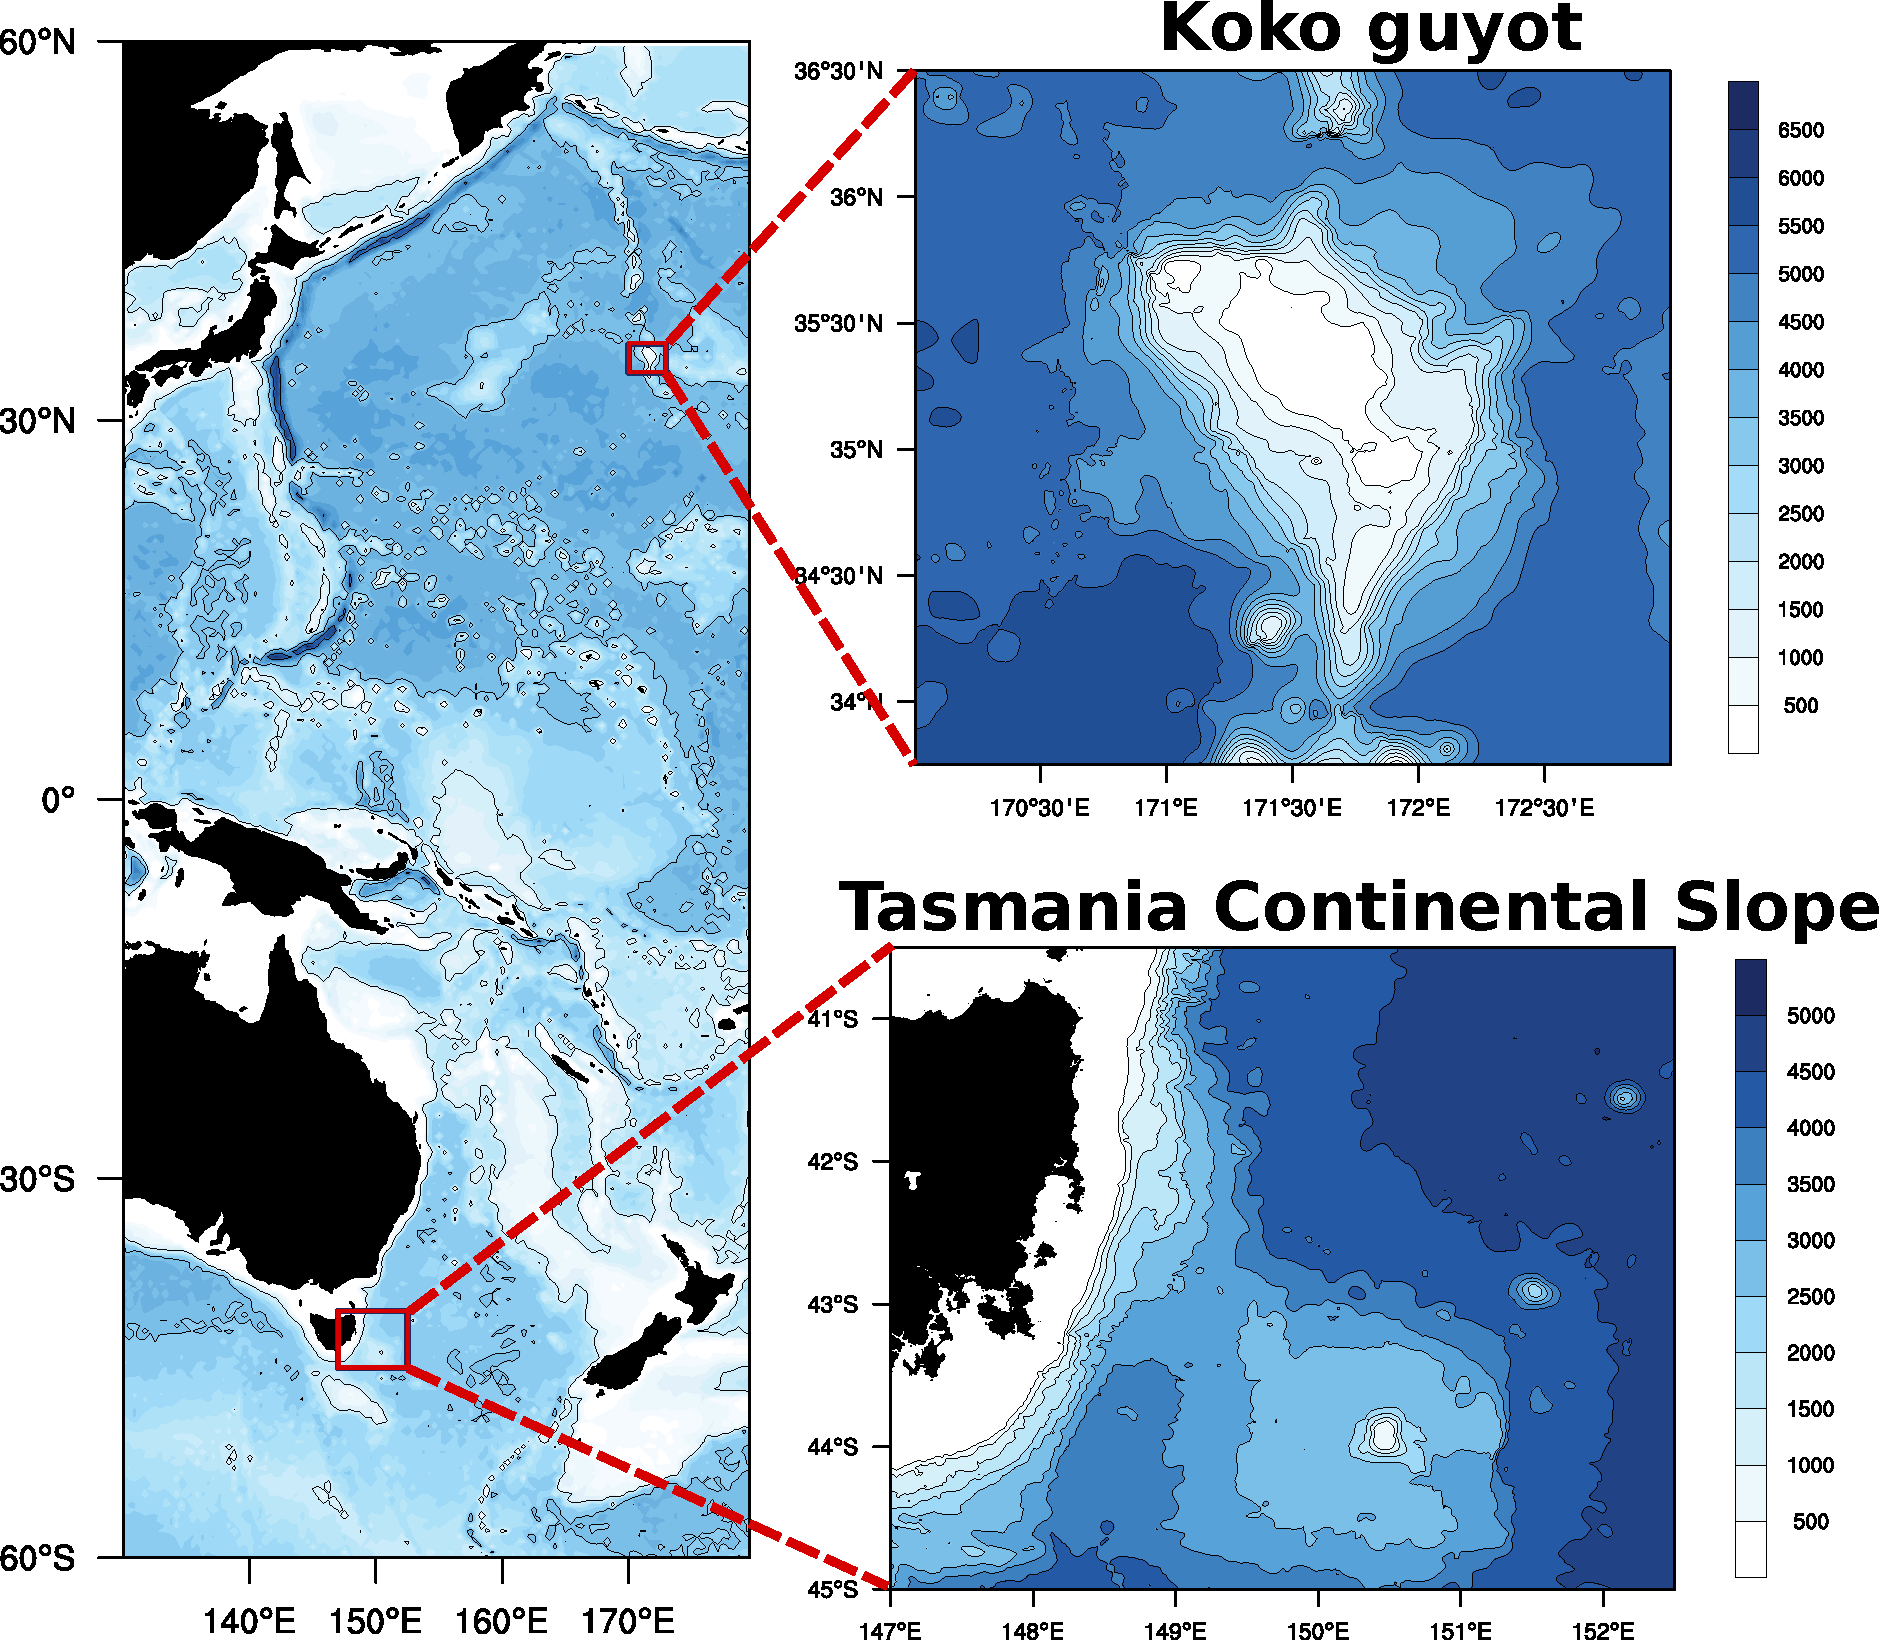
\includegraphics[scale=0.5]{../figures/map_w_places.pdf}
\caption{The map of the Pacific Ocean with outlined regions.}
\end{figure}
(\textbf{HERE IT GOES LONG INTRODUCTION to INTERNAL TIDES, GENERATION, GLOBAL SCALE, IMPORTANCE, SECTION?})\\
Another type of oscillatory motions occurring in the World Ocean is internal waves. Their existence owns to stratification of the water column. Disturbance of isopycnal surfaces create perturbations which can than freely propagate from generation region over large distances. The type of sourcing will define kinematic properties of the generated internal waves. And there is a large variety of generation mechanisms: ice keels, wind forcing, surface buoyancy forcing. Here I deal with the wave motions created by oscillatory stratified tidal flow hence making existence of internal tides. Only recently it became apparent that internal tides can transfer energy from steep topogrpahic features crossing the World Ocean and depositing their momentum creating upward motion of water column properties. Internal tides are believed to be an agent in shaping the Meridional overturning circulation.\\
Internal tides propagation characteristic and scattering properties are still poorly understand and quantified. This is a goal for Tasman Tidal Dissipation Experiment (TTIDE). Their phenomena to investigate was a scattering of internal tidal beam that crosses Tasman Sea and impinges on continental slope of Tasmania (Figure 1). The primary problem is quantifying how much energy is being reflected into the open ocean. This problem was studied by means of numerous numerical experiments. One of the major concerns presented here is a variability associated with incidence of the tidal beam, intrinsic interactions with topography and background conditions. The description of this mechanisms are useful for description of field observations and consequently creating large scale understanding of internal tide reflection which allows for more describing effects of internal tides on the World Ocean.\\
\textbf{PLUGIN: 2 TW, 1 TW, Macquarie Ridge, internal tides produce transport of particulates: sediments and can cause strong currents in deep ocean. Role in tidal dissipation, Internal tides what became apparent recently are important energy transporters.}
Both of the investigated geophysical problem represent a type of wave scattering by inhomogeneity in the media. The latter here means rapid change in ocean depth that creating conditions for wave's propagation and energetic characteristics change. As title of thesis implies the problems are dealt by application of energy considerations, mainly energy flux.

\subsection{Energy conservation and energy flux}
Even though tsunami being surface waves and internal tides are waves traveling on isopycnal surfaces they posses a similarity which enables similar treatment of their energy properties. For both cases the waves are predominantly long, their typical wavelength is much larger than the ocean's mean depth with periods longer than buoyancy period. Both tsunami and internal tides have scales of 200 km. This provides unified description by means of Laplace tidal equations on f-plane with allowance for density stratification (\cite{kundu2008fluid}, \cite{cushman2011introduction}) (or Shallow Gravity waves) which formulated as follows
\begin{align}
\pder[u]{t} - f v = -\frac{1}{\ib{\rho}_0}\pder[p]{x}\\
\pder[v]{t} + f u = -\frac{1}{\ib{\rho}_0}\pder[p]{y}\\
0 = -\pder[p]{z} - \rho g\\
N^2 w = -\frac{1}{\ib{\rho}_0} \pderr[p]{z}{t}\\
\pder[u]{x} + \pder[v]{y} + \pder[w]{z} = 0
\end{align}
with $(u,~v,~w)$ being velocity along zonal, meridional and vertical axis, $f$ - Coriolis parameter, $p$ - pressure perturbation arising from sea level or isopycnal motions of stratified water column given by Brunt-Vaisala frequency $N^2 = -\frac{g}{\ib{\rho}_0}\pder[\rho_0]{z}$. The set of equations is constructed for linear and hydrostatic flow under Boussinesq approximation. Additionally, boundary conditions are imposed on the surface (linearized) and flat bottom,
\begin{align}
w|_{z = 0} = \pder[\zeta]{t},~p|_{z = 0} = \ib{\rho}_0 g \zeta\\
w|_{z = -H} = 0
\end{align}
Such formulated problem allows separation of vertical axis by employing vertical mode decomposition,
\begin{align}
(u, v, p)(x,y,z,t) = \sum_{n = 0} [u_n(x,y,t), v_n(x,y,t), p_n(x,y,t)]\psi_n(z)\\
w(x,y,z,t) = \sum_{n = 0} [w_n(x,y,t)] \int_{-H}^z \psi_n(z) dz\\
\rho(x,y,z,t) = \sum_{n = 0} [\rho_n(x,y,t)] \frac{d \psi_n(z)}{dz}
\end{align}
Upon substitution of the decompositions Sturm-Liouville problem is obtained for vertical structure (basis) functions $\psi_n(z)$,
%\pder[\frac{1}{N^2 - \omega^2} \pder[\psi_n]{z}]{z} + \big(1 - \frac{f^2}{\omega^2} \big) \frac{\psi_n}{c^2_n} = 0
\begin{equation}
\frac{d}{dz}\big( \frac{1}{N^2} \frac{d \psi_n}{dz} \big) + \frac{1}{c^2_n}\psi_n = 0
\end{equation}
with $c_n$ being an eigenvalue for a respective $n$-th mode.\\
The carried out vertical decomposition effectively decouples vertical dynamics from horizontal reducing the initial set to shallow water-type of equations,
\begin{align}
\pder[\vec{u}_n]{t} + f \vec{k} \times \vec{u}_n = -\frac{1}{\rho_0} \nabla p_n\\
\frac{1}{\rho_0} \pder[p_n]{t} + g D_n \nabla  \cdot \vec{u}_n = 0
\end{align}
Here I intentionally introduced equivalent depth $D_n,~c_n = \sqrt{g D_n}$. For typical oceanic conditions $0$-th mode represents a barotropic solution with $\psi_0 = const$, i.e.  vertically uniform dynamics, and $D_0 \simeq H$ (\cite{hendershott1981long}. So it resembles pure surface wave propagation such as tsunami wave propagation. The left out infinite sequence of vertical modes are purely internal modes that cause isopycnal displacements of magnitude, $\eta_n = \int w dt = \int w_n \int_H^z \psi_n dz$ and negligibly small sea level motions. The latter allows complete separation between barotropic and baroclinic (vertically dependent) motions.\\
For tsunami waves due to their high frequency rotational effects are usually neglected, but can appear over long distances (Kowalik, Sumatra). Internal tides on the other hand are Sverdrup waves which are the same as long shallow water waves but perturbed with rotation causing them to be dispersive.\\
Now using framework (12-13) energy equation can be formed by multiplying momentum equations with $\vec{u}_n$ and continuity equation with $p_n$ adding both expressions and depth integrating (\cite{nekrasov1990energy}, \cite{kowalik2013oceanography}, \cite{kelly2012cascade}),
\begin{equation}
(E_k + E_p)_t + \nabla \cdot \vec{F} = D
\end{equation}

I take shallow gravity framework that works well for tsunami propagation in deep ocean. For internal tides the Boussinesq equations can be transformed into Laplace tidal equations after vertical eigenmode decomposition.\\

Energy flux appears as...\\
Nonlinearity
Since the length of continental slope is small to dominant wavelength as well as lengthscale of Koko Guoys is also small it is suffice to assume linear wave dynamics.

\subsection{Formulation of scattering problem}
Generally speaking, wave scattering happens due to inconsistency of boundary conditions. This can be expressed as the following equation.

Internal tide generation was ascribed to scattering of barotropic tidal energy from bottom relief.

\newpage
\section{TO DO}
\begin{itemize}
\item In my writing here I need to write down energy conservation equation. It must be done super careful. Ref: Wunsch, Ferrari; Nekrasov; 
\item Definition of energy flux since it is corner stone for the whole work. Ref: Kowalik papers; Nash, Kelly

\end{itemize}

\bibliographystyle{apacite}
\bibliography{/home/dmitry/Bibtex_lib/}

\end{document}